\documentclass[border=4pt]{standalone}

\usepackage{amsmath}
\usepackage{tikz}
\usepackage{mathdots}
\usepackage{yhmath}
\usepackage{cancel}
\usepackage{color}
\usepackage{siunitx}
\usepackage{array}
\usepackage{multirow}
\usepackage{amssymb}
\usepackage{gensymb}
\usepackage{tabularx}
\usepackage{booktabs}
\usetikzlibrary{fadings}
\usetikzlibrary{patterns}


\begin{document}
 
\tikzset{every picture/.style={line width=0.75pt}} %set default line width to 0.75pt

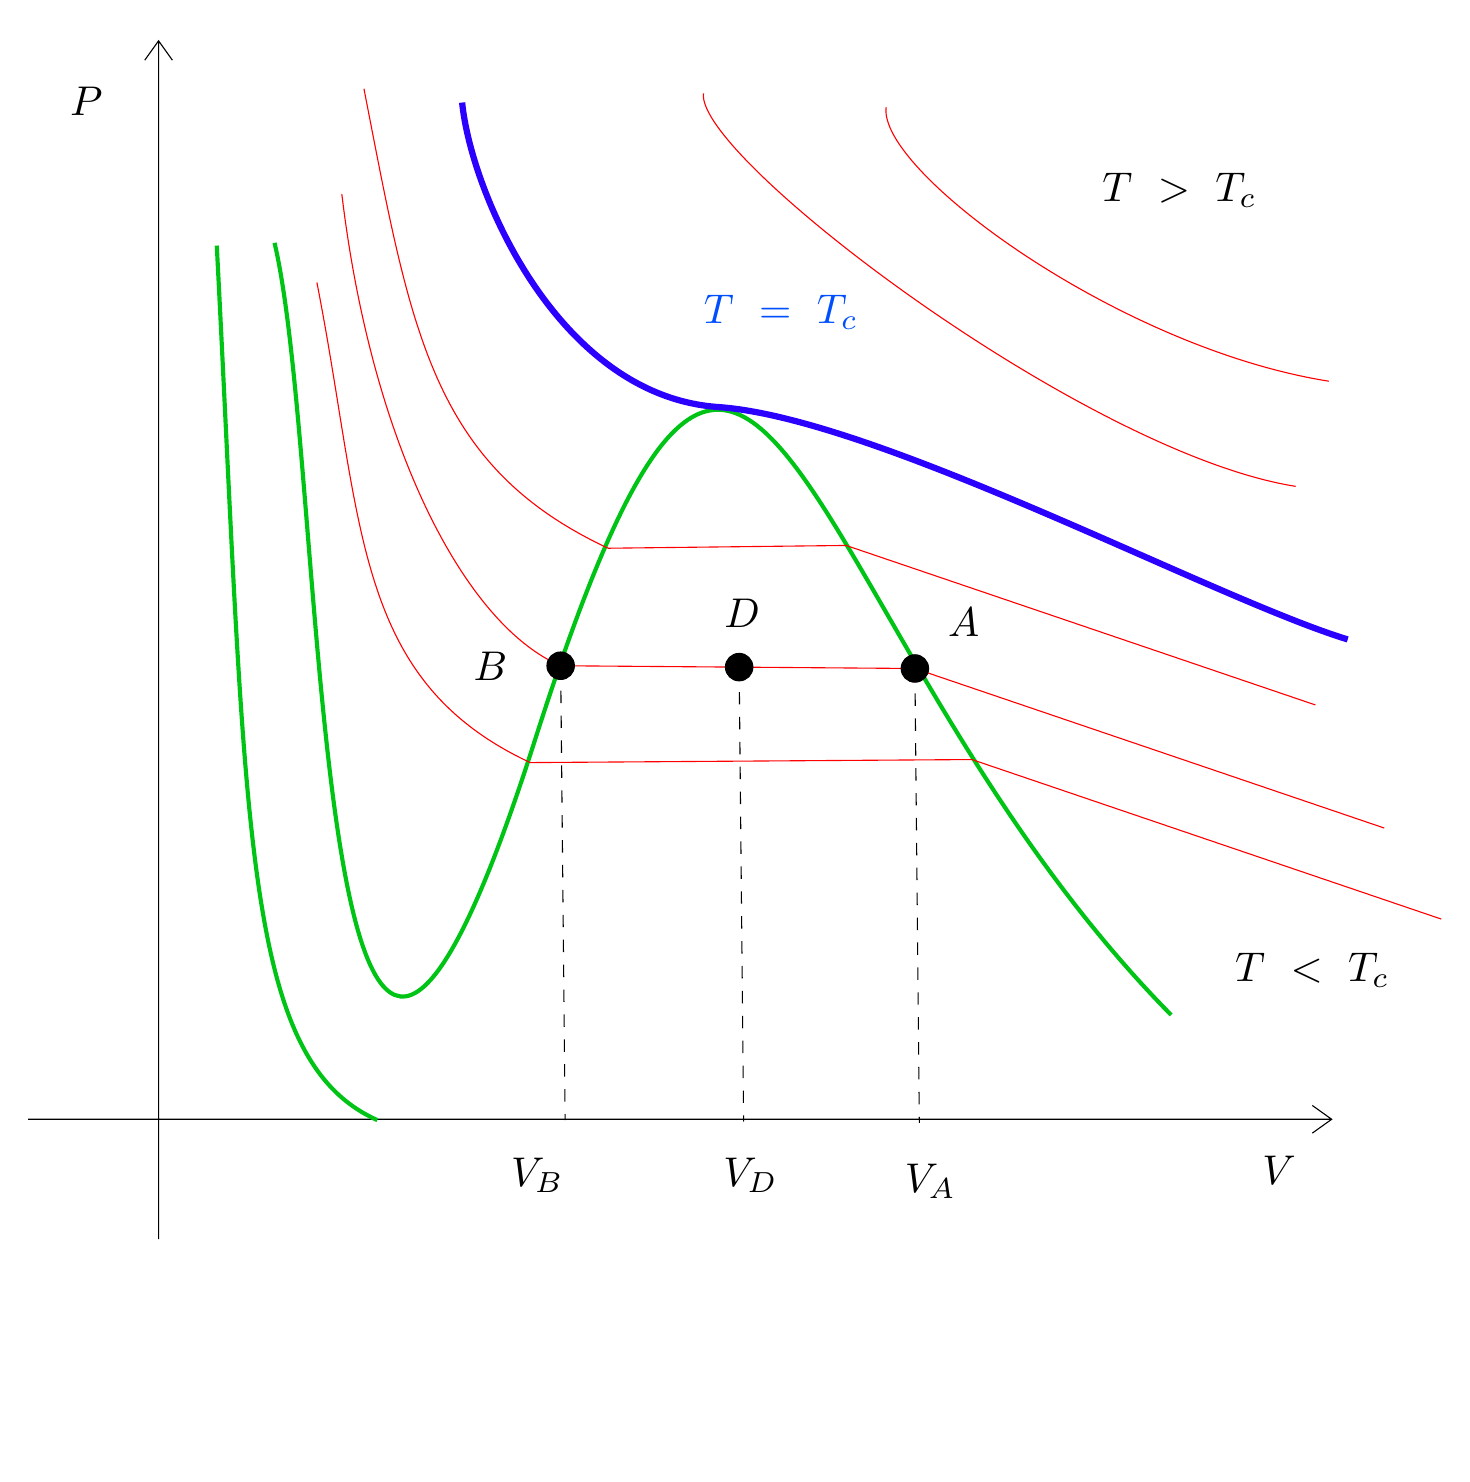
\begin{tikzpicture}[x=1pt,y=1pt,yscale=-1,xscale=1]
%uncomment if require: \path (0,433); %set diagram left start at 0, and has height of 433

%Shape: Axis 2D [id:dp34042133393206886]
\draw  (72,390.7) -- (543,390.7)(119.1,1) -- (119.1,434) (536,385.7) -- (543,390.7) -- (536,395.7) (114.1,8) -- (119.1,1) -- (124.1,8)  ;
%Straight Lines [id:da6702336744569144]
\draw  [dash pattern={on 4.5pt off 4.5pt}]  (264.39,226.81) -- (266,391) ;


%Straight Lines [id:da35901728946704126]
\draw [color={rgb, 255:red, 255; green, 0; blue, 0 }  ,draw opacity=1 ]   (263.39,226.81) -- (392.39,227.81) ;


%Curve Lines [id:da9451173727045867]
\draw [color={rgb, 255:red, 0; green, 196; blue, 21 }  ,draw opacity=1 ][line width=1.5]    (161,74) .. controls (181,159) and (173,511) .. (255,254) .. controls (337,-3) and (347,213) .. (485,353) ;


%Straight Lines [id:da08613827611481972]
\draw  [dash pattern={on 4.5pt off 4.5pt}]  (392.39,227.81) -- (394,392) ;


%Straight Lines [id:da1041450850592075]
\draw [color={rgb, 255:red, 255; green, 0; blue, 0 }  ,draw opacity=1 ]   (281.55,184.35) -- (367.55,183.35) ;


%Straight Lines [id:da726756834820412]
\draw [color={rgb, 255:red, 255; green, 0; blue, 0 }  ,draw opacity=1 ]   (253.39,261.81) -- (413.01,260.71) ;


%Straight Lines [id:da36415288687545777]
\draw  [dash pattern={on 4.5pt off 4.5pt}]  (328.89,227.31) -- (330.5,391.5) ;


%Curve Lines [id:da6577640934100049]
\draw [color={rgb, 255:red, 255; green, 0; blue, 0 }  ,draw opacity=1 ]   (193.31,18.33) .. controls (210.31,105.33) and (217.31,154.33) .. (281.55,184.35) ;


%Curve Lines [id:da5326240116615772]
\draw [color={rgb, 255:red, 255; green, 0; blue, 0 }  ,draw opacity=1 ]   (176.31,88.33) .. controls (193.31,175.33) and (189.15,231.78) .. (253.39,261.81) ;


%Curve Lines [id:da7998397977403133]
\draw [color={rgb, 255:red, 255; green, 0; blue, 0 }  ,draw opacity=1 ]   (185.31,56.33) .. controls (196.31,148.33) and (230.31,212.33) .. (264.39,226.81) ;


%Straight Lines [id:da9411455399902455]
\draw [color={rgb, 255:red, 255; green, 0; blue, 0 }  ,draw opacity=1 ]   (367.55,183.35) -- (537.13,240.99) ;


%Straight Lines [id:da28743856092342424]
\draw [color={rgb, 255:red, 255; green, 0; blue, 0 }  ,draw opacity=1 ]   (392.39,227.81) -- (561.97,285.45) ;


%Straight Lines [id:da2729807224373272]
\draw [color={rgb, 255:red, 255; green, 0; blue, 0 }  ,draw opacity=1 ]   (413.01,260.71) -- (582.59,318.35) ;


%Curve Lines [id:da846663436815342]
\draw [color={rgb, 255:red, 0; green, 196; blue, 21 }  ,draw opacity=1 ][line width=1.5]    (140.13,74.99) .. controls (151.13,285.99) and (149.13,368.99) .. (198.13,390.99) ;


%Curve Lines [id:da687077505482324]
\draw [color={rgb, 255:red, 43; green, 0; blue, 255 }  ,draw opacity=1 ][line width=2.25]    (228.79,23.31) .. controls (232.09,56.31) and (263.8,129.35) .. (321.29,133.33) .. controls (378.79,137.31) and (499.79,202.31) .. (548.79,217.31) ;


%Shape: Circle [id:dp9253191380995789]
\draw  [color={rgb, 255:red, 0; green, 0; blue, 0 }  ,draw opacity=1 ][fill={rgb, 255:red, 0; green, 0; blue, 0 }  ,fill opacity=1 ] (323.94,227.31) .. controls (323.94,224.57) and (326.15,222.35) .. (328.89,222.35) .. controls (331.63,222.35) and (333.84,224.57) .. (333.84,227.31) .. controls (333.84,230.04) and (331.63,232.26) .. (328.89,232.26) .. controls (326.15,232.26) and (323.94,230.04) .. (323.94,227.31) -- cycle ;
%Shape: Circle [id:dp4312182648745586]
\draw  [color={rgb, 255:red, 0; green, 0; blue, 0 }  ,draw opacity=1 ][fill={rgb, 255:red, 0; green, 0; blue, 0 }  ,fill opacity=1 ] (259.44,226.81) .. controls (259.44,224.07) and (261.65,221.85) .. (264.39,221.85) .. controls (267.13,221.85) and (269.34,224.07) .. (269.34,226.81) .. controls (269.34,229.54) and (267.13,231.76) .. (264.39,231.76) .. controls (261.65,231.76) and (259.44,229.54) .. (259.44,226.81) -- cycle ;
%Shape: Circle [id:dp9164322895828938]
\draw  [color={rgb, 255:red, 0; green, 0; blue, 0 }  ,draw opacity=1 ][fill={rgb, 255:red, 0; green, 0; blue, 0 }  ,fill opacity=1 ] (387.44,227.81) .. controls (387.44,225.07) and (389.65,222.85) .. (392.39,222.85) .. controls (395.13,222.85) and (397.34,225.07) .. (397.34,227.81) .. controls (397.34,230.54) and (395.13,232.76) .. (392.39,232.76) .. controls (389.65,232.76) and (387.44,230.54) .. (387.44,227.81) -- cycle ;
%Curve Lines [id:da7173087694815479]
\draw [color={rgb, 255:red, 255; green, 0; blue, 0 }  ,draw opacity=1 ]   (316,20) .. controls (313,43) and (454,150) .. (530,162) ;


%Curve Lines [id:da07422455776903614]
\draw [color={rgb, 255:red, 255; green, 0; blue, 0 }  ,draw opacity=1 ]   (382,25) .. controls (379,48) and (466,112) .. (542,124) ;



% Text Node
\draw (93,23) node  [scale=1.5]  {$P$};
% Text Node
\draw (524,409) node [scale=1.5]  {$V$};
% Text Node
\draw (256,411) node  [scale=1.5] {$V_{B}$};
% Text Node
\draw (398,413) node  [scale=1.5] {$V_{A}$};
% Text Node
\draw (333,411) node [scale=1.5]  {$V_{D}$};
% Text Node
\draw (239,227) node  [scale=1.5] {$B$};
% Text Node
\draw (410,211) node  [scale=1.5] {$A$};
% Text Node
\draw (330,208) node [scale=1.5]  {$D$};
% Text Node
\draw (344,99) node [scale=1.5] [color={rgb, 255:red, 0; green, 79; blue, 255 }  ,opacity=1 ]  {$T\ =\ T_{c}$};
% Text Node
\draw (488,55) node [scale=1.5]  {$T\  >\ T_{c}$};
% Text Node
\draw (536,337) node [scale=1.5] {$T\ < \ T_{c}$};


\end{tikzpicture}


\end{document}
